\documentclass{article}
\usepackage[utf8]{inputenc}
\usepackage[dutch]{varioref}
\usepackage[autostyle]{csquotes} 
\usepackage[dutch]{babel}
\usepackage{pdfpages}
\usepackage{natbib}
\usepackage{graphicx}

\title{Stageverslag}
\author{\mbox{Pieter-Jan} Robrecht}
\date{Maart 2016}

\begin{document}

%\maketitle
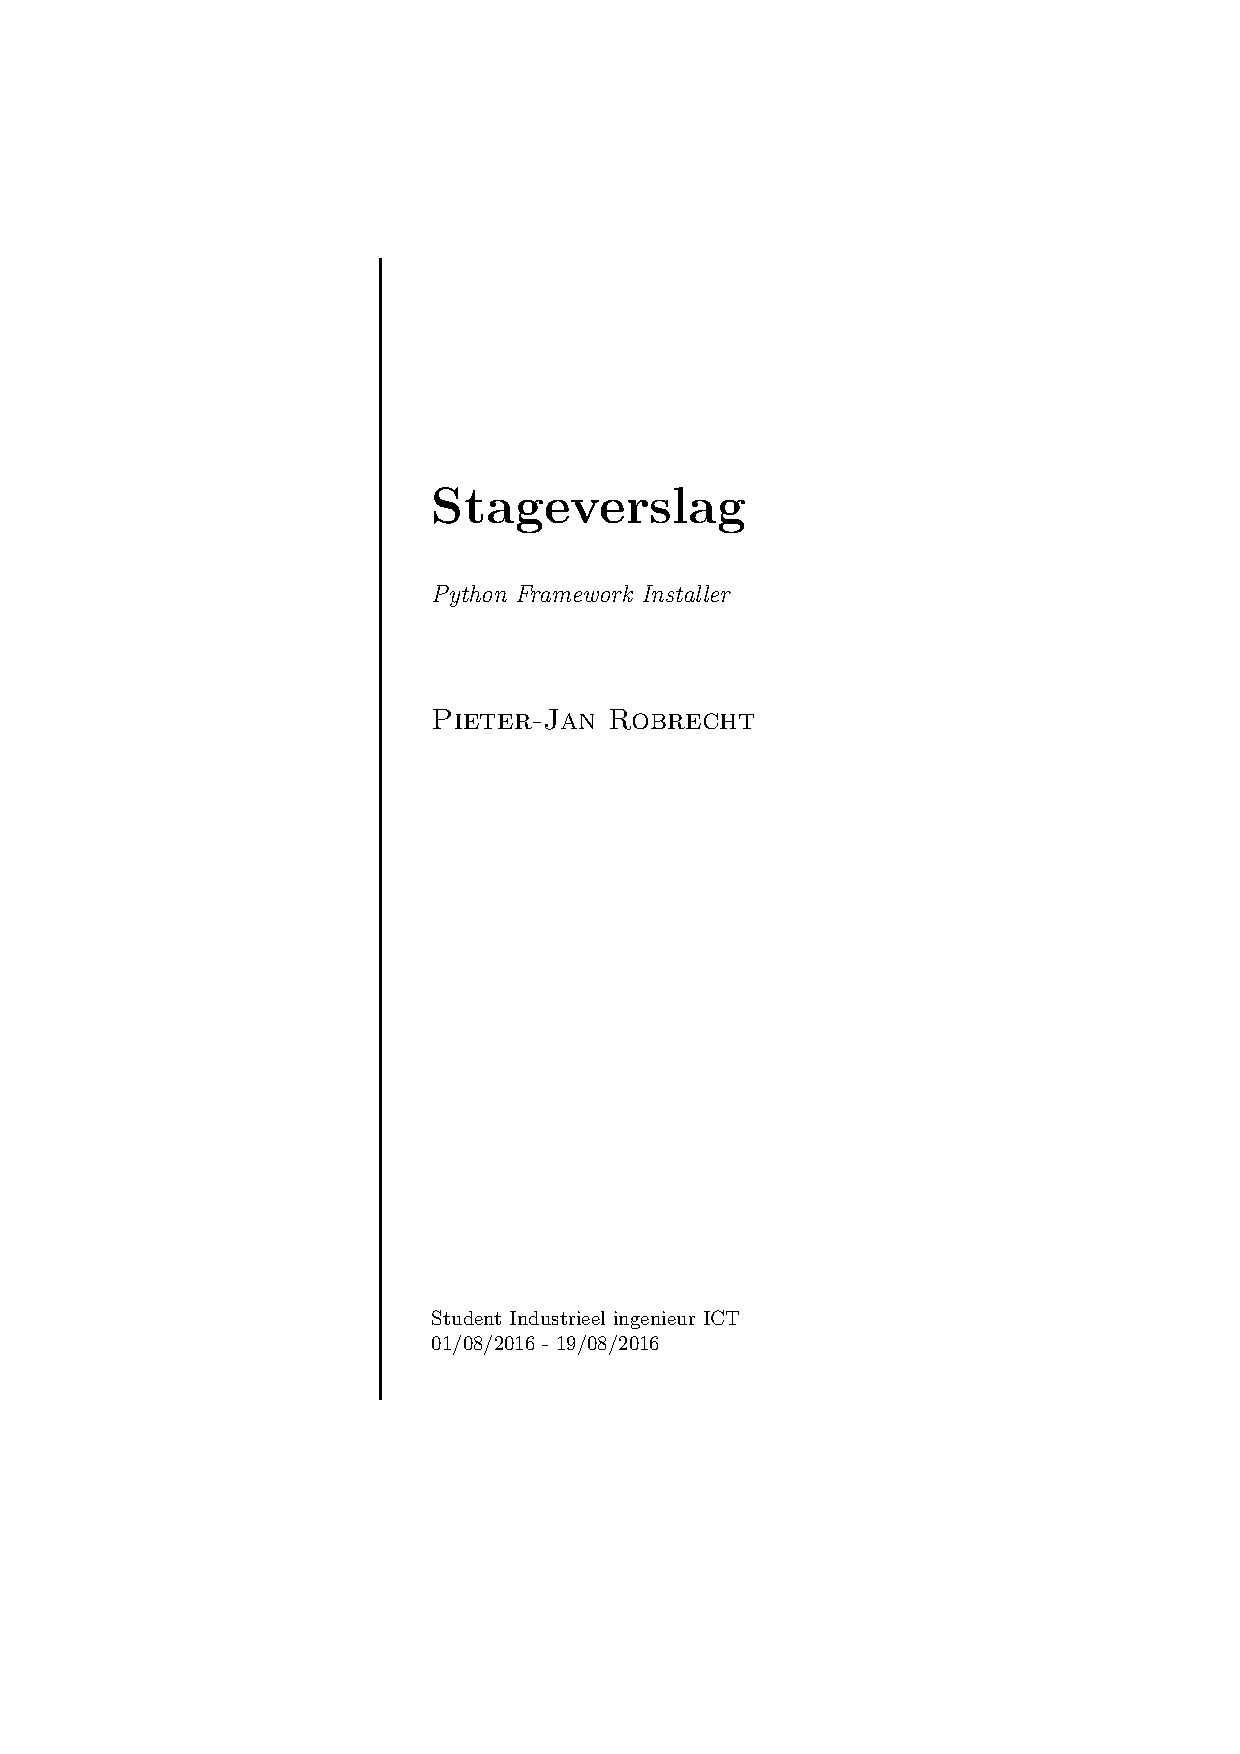
\includepdf{titel/titelstage.pdf}

%Volgende lijn is om de titelpagina geen paginanummer te geven
\clearpage
\setcounter{page}{1}

\tableofcontents
%\clearpage

\section{Inleiding}
In het kader van mijn masterproef was het mogelijk om bij Televic Rail een stage te lopen tijdens de zomer. 
Gedurende deze stage heb ik mijn masterproef voorbereid en onderzoek gedaan naar de verschillende mogelijkheden die er zijn voor het uitvoeren van mijn opdracht.
De opdracht die voltooid moet worden is de volgende:
\begin{displayquote}
Televic Rail heeft een Python test framework ontworpen. 
Dit framework werd oorspronkelijk gebruikt om gebruikt te worden op een volledig uitgeruste testtoren, maar het framework werd aangepast zodanig dat het onafhankelijk van de testtoren gebruikt kan worden.
Aangezien het framework gebruik maakt van verschillende niet-standaard Python bibliotheken, is het installeren van het framework op een nieuw systeem een hele klus.
Het doel is dan ook het maken van een installer en een updater waarmee dit proces kan worden vergemakkelijkt zodanig dat er zo min mogelijk interactie van de gebruiker moet zijn.
\end{displayquote}
Tijdens de duur van de stage werden de verschillende implementatie manieren onderzocht en werd er een algemene architectuur voor de installer-updater uitgedacht.
In wat volgt wordt er beschreven welke stappen er werden ondernomen om het probleem onder te verdelen in enkele logische stappen en hoe deze problemen dan werden opgelost. 

\section{Analyse van het probleem} \label{section:analyse}
Tijdens het bespreken van het probleem werd het al snel duidelijk dat er verschillende scenario's zijn waarin het framework gebruikt wordt. 
Het framework wordt als een standalone programma op een laptop of desktop maar het zal ook moeten draaien op verschillende testtorens. 
Voor de verschillende omgevingen zal iedere keer een andere configuratie nodig zijn maar ze wel beiden Windows gebruiken als besturingssysteem. 
Er zullen dus geen grote veranderingen moeten worden aangebracht in het maken van de installer aangezien beide omgevingen overweg kunnen met een .exe bestand. 
Uiteraard moet er rekening worden gehouden met de toekomst. 
Het framework zal in de nabije toekomst worden aangepast zodanig dat het mogelijks op een Raspberry Pi kan draaien.
Dit zou wel voor verschillende problemen kunnen zorgen aangezien een Raspberry Pi een linux distributie zal gebruiken als zijn besturingssysteem.
Aangezien linux distributies geen gebruik maken van .exe files voor het installeren van programma's zal er een alternatief worden gezocht zodanig dat het framework ook kan ge\"instaleerd kan worden op deze distributies.
Aangezien de uitbreiding naar de Raspberry Pi een toekomst plan is, gaan we hier niet de focus leggen.

Tijdens het installeren van het framework moeten we rekening houden met het feit dat iedere computer een andere configuratie en andere drivers zal nodig hebben.
Er zal een manier moeten worden uitgedacht waardoor we kunnen achterhalen welke devices zijn geconnecteerd en welke drivers deze exact nodig heeft.
Het probleem van de drivers beperkt zich jammer genoeg niet enkel tot dit.
Als er nieuwe hardware ontwikkelt wordt, zullen er ook verschillende nieuwe drivers nodig zijn. 
Voor de installer is het dan ook belangrijk dat deze nieuwe drivers snel kunnen worden toegevoegd en dat dit geen grote problemen levert.
Nieuwe versies van het framework zelf zullen ook snel en eenvoudig moeten worden gedistribueerd.

De installer is best ook een programma dat zo eenvoudig mogelijk uit te breiden is aangezien het in de toekomst nog kan worden aangepast. 
De interface naar de gebruiker toe is best ook zo eenvoudig mogelijk zodanig dat er geen problemen kunnen ontstaan tijdens de installatie van het framework.
Uiteraard gaan we er vanuit moeten gaan dat er af en toe een probleem zal ontstaan tijdens de installatie van enkele componenten.
Ook hiermee zullen we rekening moeten houden.

\section{Oplossingen}
Aangezien we een algemeen beeld hebben van wat we juist allemaal moeten voorzien, kunnen we vervolgens aan de slag met het zoeken naar een goede oplossing voor alle problemen.
In wat hierna volgt worden enkele mogelijkheden overlopen die gebruikt kunnen worden om de installer te implementeren.
Alle verschillende opties gaan overlopen worden en de verschillende voor- en nadelen zullen besproken worden.

\subsection{Mogelijkheden}
\subsubsection{WiX}
\subsubsection{NSIS}
\subsubsection{Chocolatey}
\subsection{Architectuur}

\bibliographystyle{plain}
\bibliography{bib/stagebib}

\end{document}